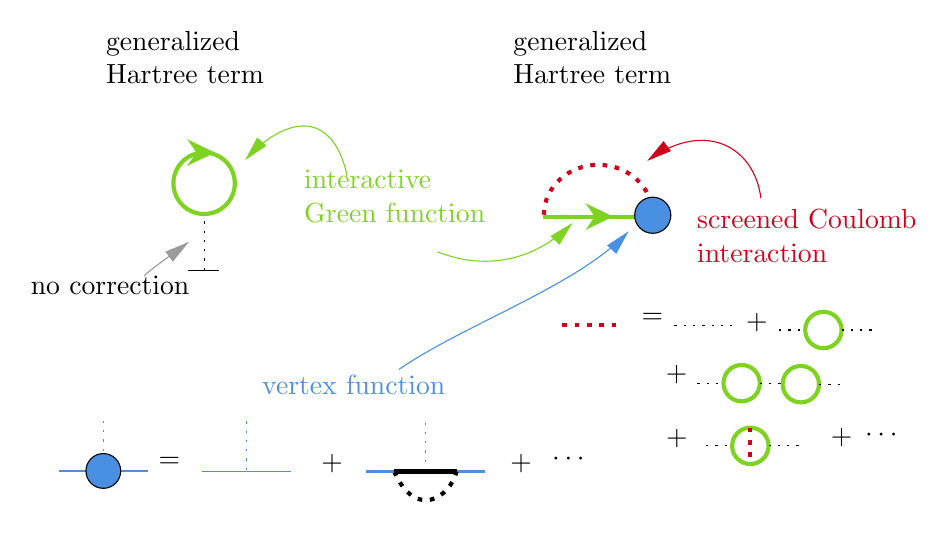
\begin{tikzpicture}[x=0.75pt,y=0.75pt,yscale=-1,xscale=1]
    %uncomment if require: \path (0,328); %set diagram left start at 0, and has height of 328
    
    %Straight Lines [id:da7829578586524399] 
    \draw    (85,132) -- (100.2,132) ;
    %Straight Lines [id:da39141889369463345] 
    \draw  [dash pattern={on 0.84pt off 2.51pt}]  (92.99,131.75) -- (92.99,104.75) ;
    %Shape: Circle [id:dp4682333299526802] 
    \draw  [color={rgb, 255:red, 126; green, 211; blue, 33 }  ,draw opacity=1 ][line width=1.5]  (78.2,89.96) .. controls (78.2,81.79) and (84.82,75.17) .. (92.99,75.17) .. controls (101.16,75.17) and (107.78,81.79) .. (107.78,89.96) .. controls (107.78,98.13) and (101.16,104.75) .. (92.99,104.75) .. controls (84.82,104.75) and (78.2,98.13) .. (78.2,89.96) -- cycle ;
    %Straight Lines [id:da20716561697715896] 
    \draw [color={rgb, 255:red, 126; green, 211; blue, 33 }  ,draw opacity=1 ][line width=1.5]    (89.82,75.15) -- (92.99,75.17) ;
    \draw [shift={(98.21,75.19)}, rotate = 180.25] [fill={rgb, 255:red, 126; green, 211; blue, 33 }  ,fill opacity=1 ][line width=0.08]  [draw opacity=0] (13.4,-6.43) -- (0,0) -- (13.4,6.44) -- (8.9,0) -- cycle    ;
    %Curve Lines [id:da17982955805390954] 
    \draw [color={rgb, 255:red, 155; green, 155; blue, 155 }  ,draw opacity=1 ]   (64.21,134.58) .. controls (64.21,133.67) and (77.81,123.96) .. (84.18,119.32) ;
    \draw [shift={(85.75,118.17)}, rotate = 143.49] [fill={rgb, 255:red, 155; green, 155; blue, 155 }  ,fill opacity=1 ][line width=0.08]  [draw opacity=0] (12,-3) -- (0,0) -- (12,3) -- cycle    ;
    %Straight Lines [id:da41757373948898713] 
    \draw [color={rgb, 255:red, 126; green, 211; blue, 33 }  ,draw opacity=1 ][line width=1.5]    (256.15,106) -- (310.48,106) ;
    \draw [shift={(290.11,106)}, rotate = 180] [fill={rgb, 255:red, 126; green, 211; blue, 33 }  ,fill opacity=1 ][line width=0.08]  [draw opacity=0] (13.4,-6.43) -- (0,0) -- (13.4,6.44) -- (8.9,0) -- cycle    ;
    %Shape: Arc [id:dp5596716734405496] 
    \draw  [draw opacity=0][dash pattern={on 1.69pt off 2.76pt}][line width=1.5]  (256.65,105.1) .. controls (256.75,91.8) and (268.47,81.06) .. (282.9,81.06) .. controls (297.39,81.06) and (309.15,91.9) .. (309.15,105.29) .. controls (309.15,105.31) and (309.15,105.33) .. (309.15,105.36) -- (282.9,105.29) -- cycle ; \draw  [color={rgb, 255:red, 208; green, 2; blue, 27 }  ,draw opacity=1 ][dash pattern={on 1.69pt off 2.76pt}][line width=1.5]  (256.65,105.1) .. controls (256.75,91.8) and (268.47,81.06) .. (282.9,81.06) .. controls (297.39,81.06) and (309.15,91.9) .. (309.15,105.29) .. controls (309.15,105.31) and (309.15,105.33) .. (309.15,105.36) ;  
    %Shape: Circle [id:dp2577884962641397] 
    \draw  [fill={rgb, 255:red, 74; green, 144; blue, 226 }  ,fill opacity=1 ] (300.44,105.36) .. controls (300.44,100.55) and (304.34,96.66) .. (309.15,96.66) .. controls (313.95,96.66) and (317.85,100.55) .. (317.85,105.36) .. controls (317.85,110.17) and (313.95,114.06) .. (309.15,114.06) .. controls (304.34,114.06) and (300.44,110.17) .. (300.44,105.36) -- cycle ;
    %Curve Lines [id:da12694407429381083] 
    \draw [color={rgb, 255:red, 208; green, 2; blue, 27 }  ,draw opacity=1 ]   (361.27,97.23) .. controls (358.13,72.15) and (334.47,59.67) .. (308.12,78.01) ;
    \draw [shift={(306.5,79.17)}, rotate = 323.47] [fill={rgb, 255:red, 208; green, 2; blue, 27 }  ,fill opacity=1 ][line width=0.08]  [draw opacity=0] (12,-3) -- (0,0) -- (12,3) -- cycle    ;
    %Straight Lines [id:da17452318018835333] 
    \draw [color={rgb, 255:red, 0; green, 0; blue, 0 }  ,draw opacity=1 ] [dash pattern={on 0.84pt off 2.51pt}]  (319.6,158.4) -- (348.1,158.4) ;
    %Straight Lines [id:da6125757076810467] 
    \draw [color={rgb, 255:red, 0; green, 0; blue, 0 }  ,draw opacity=1 ] [dash pattern={on 0.84pt off 2.51pt}]  (369.98,160.65) -- (382.6,160.65) ;
    %Shape: Circle [id:dp07446740538840513] 
    \draw  [color={rgb, 255:red, 126; green, 211; blue, 33 }  ,draw opacity=1 ][line width=1.5]  (382.6,160.65) .. controls (382.6,155.81) and (386.53,151.88) .. (391.37,151.88) .. controls (396.21,151.88) and (400.14,155.81) .. (400.14,160.65) .. controls (400.14,165.49) and (396.21,169.42) .. (391.37,169.42) .. controls (386.53,169.42) and (382.6,165.49) .. (382.6,160.65) -- cycle ;
    %Straight Lines [id:da8816369094187908] 
    \draw [color={rgb, 255:red, 0; green, 0; blue, 0 }  ,draw opacity=1 ] [dash pattern={on 0.84pt off 2.51pt}]  (400.14,160.65) -- (415.23,160.65) ;
    %Straight Lines [id:da8976339340793376] 
    \draw [color={rgb, 255:red, 0; green, 0; blue, 0 }  ,draw opacity=1 ] [dash pattern={on 0.84pt off 2.51pt}]  (330.58,186.25) -- (343.2,186.25) ;
    %Shape: Circle [id:dp03983589213496108] 
    \draw  [color={rgb, 255:red, 126; green, 211; blue, 33 }  ,draw opacity=1 ][line width=1.5]  (343.2,186.25) .. controls (343.2,181.41) and (347.13,177.48) .. (351.97,177.48) .. controls (356.81,177.48) and (360.74,181.41) .. (360.74,186.25) .. controls (360.74,191.09) and (356.81,195.02) .. (351.97,195.02) .. controls (347.13,195.02) and (343.2,191.09) .. (343.2,186.25) -- cycle ;
    %Straight Lines [id:da7664747442145097] 
    \draw [color={rgb, 255:red, 0; green, 0; blue, 0 }  ,draw opacity=1 ] [dash pattern={on 0.84pt off 2.51pt}]  (360.74,186.25) -- (373.58,186.25) ;
    %Shape: Circle [id:dp7441999244158157] 
    \draw  [color={rgb, 255:red, 126; green, 211; blue, 33 }  ,draw opacity=1 ][line width=1.5]  (371.7,186.75) .. controls (371.7,181.91) and (375.63,177.98) .. (380.47,177.98) .. controls (385.31,177.98) and (389.24,181.91) .. (389.24,186.75) .. controls (389.24,191.59) and (385.31,195.52) .. (380.47,195.52) .. controls (375.63,195.52) and (371.7,191.59) .. (371.7,186.75) -- cycle ;
    %Straight Lines [id:da9405102182375402] 
    \draw [color={rgb, 255:red, 0; green, 0; blue, 0 }  ,draw opacity=1 ] [dash pattern={on 0.84pt off 2.51pt}]  (389.24,186.75) -- (401.87,186.75) ;
    %Straight Lines [id:da932289713688178] 
    \draw [color={rgb, 255:red, 208; green, 2; blue, 27 }  ,draw opacity=1 ][line width=1.5]  [dash pattern={on 1.69pt off 2.76pt}]  (265.6,158.4) -- (294.1,158.4) ;
    %Curve Lines [id:da7186061820300091] 
    \draw [color={rgb, 255:red, 74; green, 144; blue, 226 }  ,draw opacity=1 ]   (186.87,179.63) .. controls (218.39,157.96) and (271.87,139.66) .. (296.4,114.26) ;
    \draw [shift={(297.5,113.1)}, rotate = 132.71] [fill={rgb, 255:red, 74; green, 144; blue, 226 }  ,fill opacity=1 ][line width=0.08]  [draw opacity=0] (12,-3) -- (0,0) -- (12,3) -- cycle    ;
    %Straight Lines [id:da8405221465444168] 
    \draw [line width=1.5]    (184.56,228.8) -- (199.6,228.8) ;
    %Straight Lines [id:da7289358295015977] 
    \draw [color={rgb, 255:red, 74; green, 144; blue, 226 }  ,draw opacity=1 ] [dash pattern={on 0.84pt off 2.51pt}]  (199.6,205.22) -- (199.6,228.8) ;
    %Straight Lines [id:da31332828037117166] 
    \draw [color={rgb, 255:red, 74; green, 144; blue, 226 }  ,draw opacity=1 ][line width=0.75]    (214.64,228.8) -- (228.31,228.8) ;
    %Curve Lines [id:da08739725558309086] 
    \draw [line width=1.5]  [dash pattern={on 1.69pt off 2.76pt}]  (184.56,228.8) .. controls (195.06,252.38) and (211.31,241.38) .. (214.64,228.8) ;
    %Straight Lines [id:da045219019820437856] 
    \draw [color={rgb, 255:red, 0; green, 0; blue, 0 }  ,draw opacity=1 ] [dash pattern={on 0.84pt off 2.51pt}]  (334.78,216.45) -- (347.4,216.45) ;
    %Shape: Circle [id:dp8905022860401997] 
    \draw  [color={rgb, 255:red, 126; green, 211; blue, 33 }  ,draw opacity=1 ][line width=1.5]  (347.4,216.45) .. controls (347.4,211.61) and (351.33,207.68) .. (356.17,207.68) .. controls (361.01,207.68) and (364.94,211.61) .. (364.94,216.45) .. controls (364.94,221.29) and (361.01,225.22) .. (356.17,225.22) .. controls (351.33,225.22) and (347.4,221.29) .. (347.4,216.45) -- cycle ;
    %Straight Lines [id:da10316693133402732] 
    \draw [color={rgb, 255:red, 0; green, 0; blue, 0 }  ,draw opacity=1 ] [dash pattern={on 0.84pt off 2.51pt}]  (364.94,216.45) -- (380.03,216.45) ;
    %Straight Lines [id:da344206518292548] 
    \draw [color={rgb, 255:red, 208; green, 2; blue, 27 }  ,draw opacity=1 ][line width=1.5]  [dash pattern={on 1.69pt off 2.76pt}]  (356.17,207.68) -- (356.17,225.22) ;
    %Straight Lines [id:da9189136605818791] 
    \draw [line width=1.5]    (199.6,228.8) -- (214.64,228.8) ;
    %Straight Lines [id:da8740616138093633] 
    \draw [color={rgb, 255:red, 74; green, 144; blue, 226 }  ,draw opacity=1 ][line width=0.75]    (170.89,228.8) -- (184.56,228.8) ;
    %Straight Lines [id:da5459710428076923] 
    \draw [color={rgb, 255:red, 74; green, 144; blue, 226 }  ,draw opacity=1 ]   (23.06,228.55) -- (36.06,228.55) ;
    %Straight Lines [id:da13994557764632876] 
    \draw [color={rgb, 255:red, 74; green, 144; blue, 226 }  ,draw opacity=1 ]   (52.81,228.55) -- (65.81,228.55) ;
    %Shape: Circle [id:dp9752820209547781] 
    \draw  [fill={rgb, 255:red, 74; green, 144; blue, 226 }  ,fill opacity=1 ] (36.06,228.55) .. controls (36.06,223.92) and (39.81,220.17) .. (44.43,220.17) .. controls (49.06,220.17) and (52.81,223.92) .. (52.81,228.55) .. controls (52.81,233.18) and (49.06,236.92) .. (44.43,236.92) .. controls (39.81,236.92) and (36.06,233.18) .. (36.06,228.55) -- cycle ;
    %Straight Lines [id:da6237256272311238] 
    \draw [color={rgb, 255:red, 74; green, 144; blue, 226 }  ,draw opacity=1 ] [dash pattern={on 0.84pt off 2.51pt}]  (44.43,204.38) -- (44.43,220.17) ;
    %Straight Lines [id:da5304329557160252] 
    \draw [color={rgb, 255:red, 74; green, 144; blue, 226 }  ,draw opacity=1 ]   (92.06,228.8) -- (113.43,228.8) ;
    %Straight Lines [id:da4194355801541212] 
    \draw [color={rgb, 255:red, 74; green, 144; blue, 226 }  ,draw opacity=1 ]   (113.43,228.8) -- (134.81,228.8) ;
    %Straight Lines [id:da27508665266523624] 
    \draw [color={rgb, 255:red, 74; green, 144; blue, 226 }  ,draw opacity=1 ] [dash pattern={on 0.84pt off 2.51pt}]  (113.43,204.63) -- (113.43,228.13) ;
    %Curve Lines [id:da25752133963430035] 
    \draw [color={rgb, 255:red, 126; green, 211; blue, 33 }  ,draw opacity=1 ]   (161.88,86.33) .. controls (155.1,55.22) and (133.63,56.68) .. (113.95,77.45) ;
    \draw [shift={(112.75,78.75)}, rotate = 312.27] [fill={rgb, 255:red, 126; green, 211; blue, 33 }  ,fill opacity=1 ][line width=0.08]  [draw opacity=0] (12,-3) -- (0,0) -- (12,3) -- cycle    ;
    %Curve Lines [id:da33582469284216643] 
    \draw [color={rgb, 255:red, 126; green, 211; blue, 33 }  ,draw opacity=1 ]   (205.46,123) .. controls (220.16,128.88) and (245.9,132.6) .. (269.08,110.39) ;
    \draw [shift={(270.5,109)}, rotate = 134.75] [fill={rgb, 255:red, 126; green, 211; blue, 33 }  ,fill opacity=1 ][line width=0.08]  [draw opacity=0] (12,-3) -- (0,0) -- (12,3) -- cycle    ;
    
    % Text Node
    \draw (8.25,133.25) node [anchor=north west][inner sep=0.75pt]   [align=left] {no correction};
    % Text Node
    \draw (44.5,15.25) node [anchor=north west][inner sep=0.75pt]   [align=left] {generalized \\Hartree term};
    % Text Node
    \draw (240.75,15.25) node [anchor=north west][inner sep=0.75pt]   [align=left] {generalized \\Hartree term};
    % Text Node
    \draw (329.3,101.37) node [anchor=north west][inner sep=0.75pt]  [color={rgb, 255:red, 208; green, 2; blue, 27 }  ,opacity=1 ] [align=left] {screened Coulomb \\interaction};
    % Text Node
    \draw (352.85,151.15) node [anchor=north west][inner sep=0.75pt]   [align=left] {+};
    % Text Node
    \draw (314.2,176.5) node [anchor=north west][inner sep=0.75pt]   [align=left] {+};
    % Text Node
    \draw (302.56,151.15) node [anchor=north west][inner sep=0.75pt]   [align=left] {=};
    % Text Node
    \draw (314.32,207.28) node [anchor=north west][inner sep=0.75pt]   [align=left] {+};
    % Text Node
    \draw (393.65,206.62) node [anchor=north west][inner sep=0.75pt]   [align=left] {+};
    % Text Node
    \draw (410.23,207.03) node [anchor=north west][inner sep=0.75pt]   [align=left] {$\displaystyle \cdots $};
    % Text Node
    \draw (119.7,181.37) node [anchor=north west][inner sep=0.75pt]  [color={rgb, 255:red, 208; green, 2; blue, 27 }  ,opacity=1 ] [align=left] {\textcolor[rgb]{0.29,0.56,0.89}{vertex function}};
    % Text Node
    \draw (69.81,220.55) node [anchor=north west][inner sep=0.75pt]    {$=$};
    % Text Node
    \draw (148.23,219.22) node [anchor=north west][inner sep=0.75pt]   [align=left] {+};
    % Text Node
    \draw (239.23,219.22) node [anchor=north west][inner sep=0.75pt]   [align=left] {+};
    % Text Node
    \draw (259.43,218.63) node [anchor=north west][inner sep=0.75pt]   [align=left] {$\displaystyle \cdots $};
    % Text Node
    \draw (139.96,82.5) node [anchor=north west][inner sep=0.75pt]  [color={rgb, 255:red, 126; green, 211; blue, 33 }  ,opacity=1 ] [align=left] {interactive \\Green function};
    
    
    \end{tikzpicture}
    